
\section{PAMELA approach for specification and run-time monitoring of cyber-contracts}
%\section{Experiments and preliminary evaluation}

\cite{guerin:hal-03217126}

\cite{silva:hal-02958111}

In this section, we show how our approach can be mapped on two frameworks to specify cyber-contracts on security patterns and we show how to use them on existing code.
%This section discusses the implementation of our approach in two different languages as well as a preliminary evaluation study.

In particular, our approach was implemented in two software specification languages. Both implementations enable the addition of an extra layer of trust in the existing code, to enforce the formal properties of predefined security design patterns, without the need to modify the code. We implemented our approach in the Java Modelling Language (JML) \cite{leavens2006}, a DbC-based specification language, and PAMELA, a Java modelling language and framework \cite{PAMELAWebSite}.

These two languages were selected on the basis of an existing active community, the relevance regarding our approach and their ability to be extended without having to enrich or modify the syntax of the hosting language.

\subsection{Java modelling language experiment}
%Our design by contract approach to specify security patterns was implemented in two software specification languages. In particular, both implementations enable the addition of an extra layer of trust in the code of a system to enforce the formal properties of existing security design patterns without the need to modify the code. We implemented our approach in the Java Modelling Language (JML), a DbC-based specification language, and PAMELA, a framework to ...
%These two languages were selected on the basis of their popularity and their ability to be extended without having to enrich or modify the syntax of the language.
%We started from the observation that in most cases, existing code implements forms of security patterns without naming them. The objective was therefore to develop to show that it was possible to start from an existing code and secure it without much modification. The securing in question is of course linked to the notion of contracts. I therefore followed two successive approaches to secure existing code. The first approach consists in implementing the contracts with JML (Java Modelling Language). The second is the implementation of security patterns in the PAMELA framework.

%\subsubsection{Java modelling language implementation}
Java Modelling Language (JML) \cite{leavens2006,cok2014} is a specification language  that enables engineers to write DbC assertions as comments in Java code. These comments are then parsed by a specific compiler (called JMLC). The resulting java bytecode is the aggregation of java compile code and java assertions enforcing JML expressions.
The JML language allows referencing the namespace of the Java program and the logical operators of the Java language. It also has some keywords and symbols that correspond, for the most part, to the concepts of the DbC approach. For example:
\begin{itemize}
    \item \textit{forall}, \textit{exist}, $=>$ and $<=>$, which correspond to the universal quantification, existential quantification, and logical implication and equivalence, respectively;
    \item \textit{invariant}, \textit{requires} and \textit{ensures} are used to represent, respectively, the invariants, preconditions and postconditions of contracts;
    \item assignable \textit{<name>} to specify that a variable can be assigned in the method it specifies;;
    \item \textit{old<name>} to reference the value of a variable before the call of the method it specifies;
    \item \textit{result} to reference the return value of the method it specifies;
    \item \textit{signals} describes the exceptions thrown by the method it specifies;
    \item \textit{pure} specifies that the specified method does not have side effects;
    \item \textit{also}: declares that a method inherits JML specification (preconditions and postconditions) from its supertype and adds specific specifications.
\end{itemize}

We use OpenJML \cite{cok2014} as the tool support to create the logical annotations in existing Java programs. In addition, it enables static or run-time checking of the validity of the annotations through static code verification and dynamic assertion checking capabilities.
%Pas sur de comprendre ce que tu veux dire par là. JML est le langage, JMLC le compilateur et openJML le framework qui permet de faire de la vérification formelle sur du code JML.


The rest of this subsection shows how to specify the \textit{Authenticator} pattern as a cyber-security contract with JML and some lessons learned from this experience. 

To specify the \textit{Authenticator} pattern as a cyber-security contract with JML, the six formal properties presented in Section \ref{label:authenticatorContract} are implemented through JML expressions, as presented below:
\begin{enumerate}
    \item Uniqueness of authentication information
    \begin{equation*}
        P1: \forall a, b \in I_{Subject},a \ne b \implies a.authInfo  \ne b.authInfo 
    \end{equation*}
    This property illustrates one of the limitations of the standard DbC approach and consequently the JML framework, in which a property is limited to be expressed for the scope of a class or a method, and so relative to one instance. As a result, this property cannot be expressed in JML since a JML expression is limited to the scope of a class and cannot involve more than one instance of the corresponding class.
    %To overcome this constraint, the code of the pattern must be expanded on adding code which impact the pattern classes.
    
    \item Invariance of authentication information
    \begin{equation*}
        P2: \forall a \in I_{Subject}, a.authInfo = a.authInfo_{ini}
    \end{equation*}
    This property is conceptually an invariant of the \textit{Subject} class. It however requires to know, at all time, what is the initial value of the \textit{authenticationInformation} field. One way to implement this "memory" in JML is to add the following ensure clause to every method, except the constructor, of the \textit{Subject} class. The constructor call does not support the use of $\backslash$old(authInfo) keyword. This is why we cannot use an invariant clause.
    \begin{center}
        \textit{@ ensures authInfo == $\backslash$old(authInfo);}
    \end{center}
    
    \item Invariance of authenticator
    \begin{equation*}
        P3: \forall a \in I_{Subject}, a.authenticator = a.authenticator_{ini}
    \end{equation*}
    This property can be implemented similarly to the previous one with the following ensure clause for every method of the \textit{Subject} class.
    \begin{center}
        \textit{@ ensures authenticator == $\backslash$old(authenticator);}
    \end{center}
    
    \item Validity of the Proof of Identity
    \begin{equation*}
    \begin{split}
        &P4: \forall a \in I_{Subject}, (a.idProof = \emptyset) \lor \\&(a.idProof = a.authenticator.request(a.authInfo))
    \end{split}
    \end{equation*}
    This property can be transposed to the following JML invariant for the \textit{Subject} class.
    \begin{center}
        \textit{@ invariant idProof == null || idProof == authenticator.request(authInfo);}
    \end{center}
    
    \item Correctness of authenticate method
    \begin{equation*}
        P5: self.idProof = self.authenticator.request(self.authInfo)
    \end{equation*}
    This property is directly a JML postcondition for the \textit{authenticate} method of the \textit{Subject} class.
    \begin{center}
        \textit{@ ensures idProof == authenticator.request(authInfo);}
    \end{center}
    
    \item Correctness of the request method
    \begin{equation*}
        P6: self.check(authInfo) \lor returnValue = \emptyset
    \end{equation*}
    This property is also a JML postcondition for the \textit{request} method of the \textit{Authenticator} class.
     \begin{center}
        \textit{@ ensures check(authInfo)} || \textit{$\backslash$result == null;}
    \end{center}
\end{enumerate}

%JML Implementation results and lessons learned
Regarding our approach, the previous example highlights the limitations of the standard DbC approach and consequently the JML framework. More specifically, there are two main expression issues that cannot be solved. The first is the limitation of a JML contract to the scope of a class or a method . This restriction prevents the expression of any contract property involving more than one instance of a class. The second issue has to do with the lack of memory of the JML-based DbC approach. Indeed, in JML, a DbC property can only refer to the current state of an instance, or in the case of the post or precondition of a method, to the state before the call of the method. The previous examples show that we sometimes need to have an evolving state for the scope of the contract properties. This could be managed for instance by implementing pattern objects that could enforce the contract properties. 
% ?? (retiré sans être sur mais ici on donne la solution de Pamela) In particular, these objects would have an evolving state and could therefore save any information relevant to their associated contract properties and at any moment of the execution.
%Caine: Generalize as to what the limitations of JML-based properties are. 

\subsection{The PAMELA experiment}

%\subsubsection{The PAMELA framework}

PAMELA is a Java modelling framework developed by the Openflexo community \footnote{https://www.openflexo.org}. This project aims at bridging the gap between software modelling and code implementation. 
%In the context of Model-Driven Engineering (MDE), the generative approach is promoted from a domain model to a dedicated model or a custom application source code. 
% TODO: @Joel: que veux-tu dire là ???
%This gap includes generally a semantic gap, because semantics may be hidden or remains implicit in the transformation. %Another drawback is the development or maintenance process, where model and source code must evolve independently and complex round-tripping mechanisms must be enforced. 

In this context, PAMELA modelling framework proposes an approach where models are directly weaved in source code, by means of Java annotations. Thus, it does not require code generation. That way, both model and source-code coexist in the same artifact. 
%A major challenge to be addressed by MDE approaches is the ability to integrate custom implementation to a base of code derived from a domain model. 
%PAMELA framework allows the use of common extension points such as inheritance, as offered by the Java language, and provides a way to define some partial implementations (a set of methods), easing coupling between formal behaviour as specified in the domain model, and custom implementations.
%PAMELA framework provides a way to define a domain model and its associated code separately from the application code. 
%The annotation support allows an easy and flexible coupling of the specified domain model and custom implementation.

\begin{figure}
    \centering
    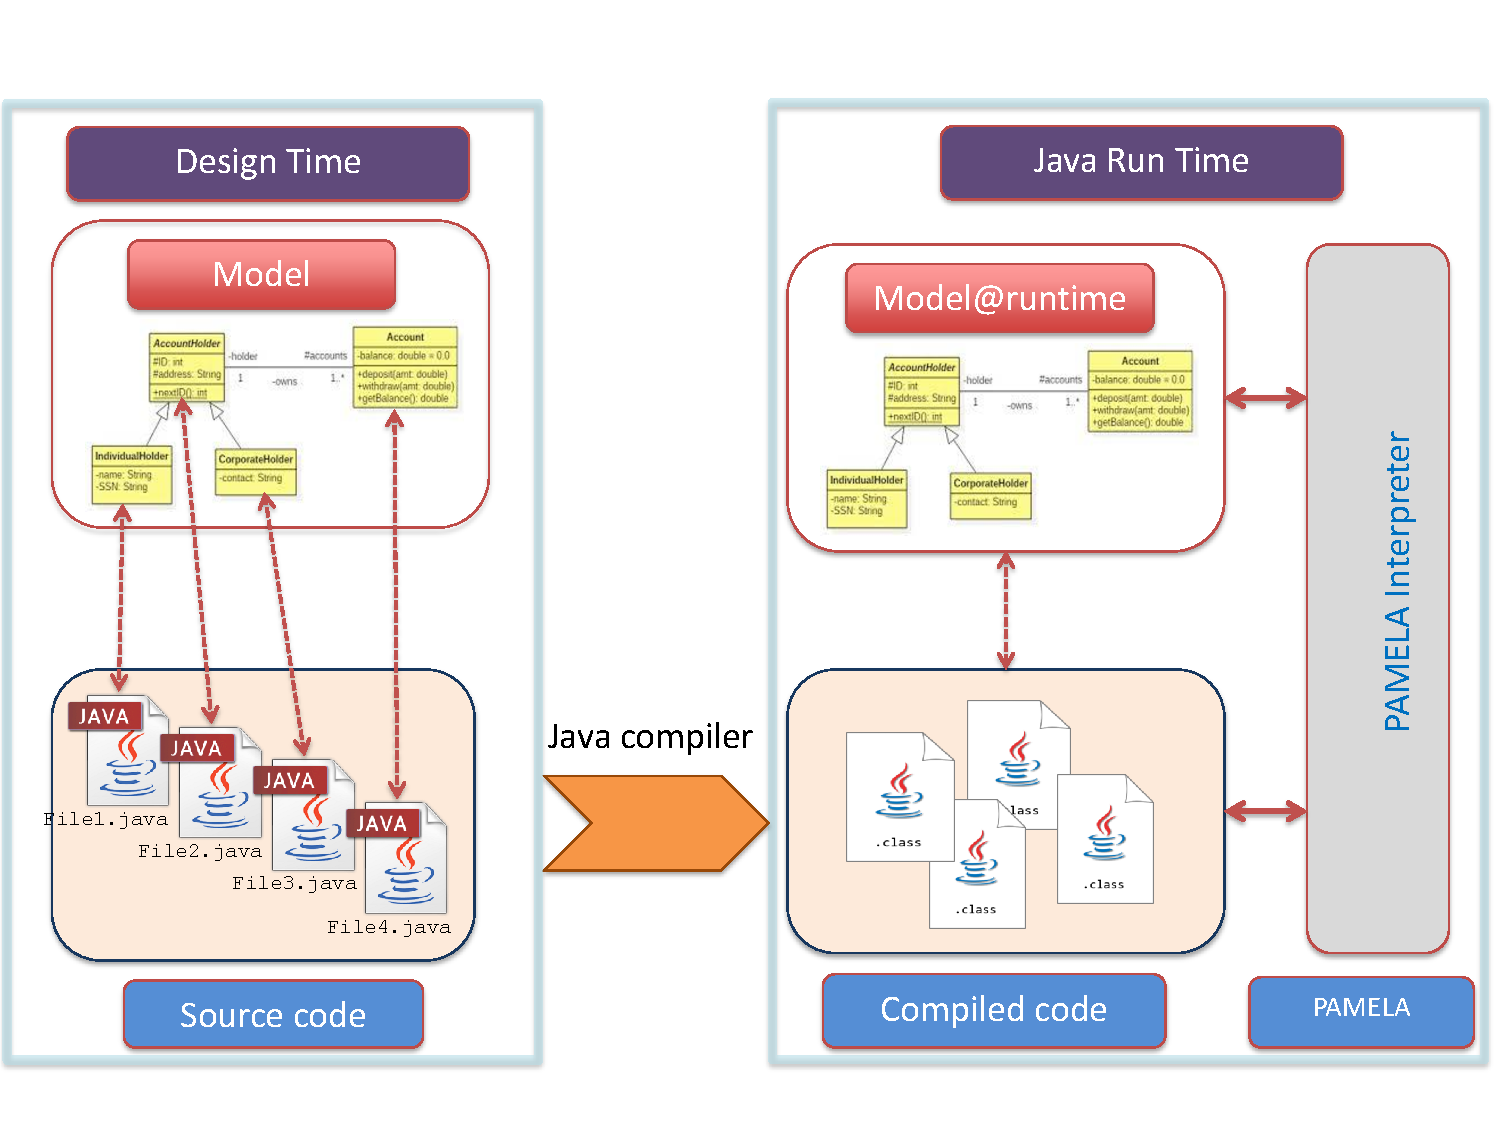
\includegraphics[width=1.0 \columnwidth]{utils/PamelaVisionV2.pdf}
    \caption{Overview of the PAMELA approach}
    \label{fig:PamelaVision}
\end{figure}

Figure \ref{fig:PamelaVision} illustrates the PAMELA framework where we have at design time (left side of the figure), the model weaved in source code files based on the Java annotations and at run-time (right side of the figure) the PAMELA interpreter ensuring the link between the model behavior and the application Java byte-code.

Resulting execution is a combination of (i) executing plain Java byte-code as the result of the basic compilation of source code, and (ii) an embedded PAMELA interpreter executing PAMELA model semantics.
 
From an implementation standpoint, PAMELA uses \emph{javassist} reflection library including the \texttt{MethodHandler} mechanism. Based on this support, the Java dynamic binding is overridden to provide the call of the PAMELA model behavior when an object method is invoked. 
%which is part of a PAMELA model caused the real implementation to be called when existing (more precisely dispatch code execution between all provided implementations), or the required interpretation according to underlying model to be executed. This provides also an extension point allowing to instrument the code, which is used for other features such as undo/redo stack management, and allows assertion checking at run-time. PAMELA framework is a 100\% pure Java (> 1.5), compilable by a classical Java compiler and executable in a classical Java virtual machine.


%\subsubsection{PAMELA \emph{Patterns}}

PAMELA framework offers some Aspect-Oriented Programming (AOP) features enabling the definition of additional behaviour to existing Java code. 

%We define a \emph{Pattern} as a composite of multiple stakeholders, whose roles are played by various Java classes. A \emph{Pattern} regroup and implement all concerns related to concept association, which are orthogonal to each functional class concern. Each method of involved classes can be considered as a \emph{pointcut} as of AOP terminology. Such \emph{Pattern} is instantiated, and provides a statefull environment. Code instrumentation and code weaving are operated at run-time by PAMELA interpreter. A \emph{Pattern} comes with its business logic (acting on control flow of all pattern-related methods), and a set of assertions (invariants, pre-conditions and post-conditions) which are evaluated at run-time, while functional code is executed.

%We choose to implement our approach with PAMELA \emph{Patterns} because this scheme perfectly fits our requirements:
%\begin{itemize}
%    \item the ability to use existing plain Java code, without any restriction,
%    \item existing code can be instrumented (PAMELA provide handlers both at entry and exit of methods execution, allowing execution of pre and post conditions),
%    \item pattern can offer some structural and behavioural features, executed by PAMELA interpreter, 
%    \item patterns are instantiated and provides statefull environment, allowing the computation of assertions using many paradigms (e.g., Linear Temporal Logic),
%    \item PAMELA offers multiple extension points: ability to redefine or specialize an existing pattern, and ability to provide a new pattern definition.
%\end{itemize}

We chose to extend the PAMELA framework to include our notion of \emph{Pattern}, i.e. a composition of multiple classes, known as \emph{Stakeholders}, whose expected behavior is defined in a pattern contract, along with formal properties which must be ensured at run-time. More specifically, implementing \emph{Patterns} with PAMELA provides:
\begin{itemize}
    \item the ability to use existing plain Java code, without any restriction;
    \item the ability to monitor the execution of the code;
    \item the ability to offer extra structural and behavioral features, executed by the PAMELA interpreter;
    \item a representation of \emph{Patterns} as stateful objects. Such objects can then evolve throughout run-time and compute assertions using any paradigms (e.g., LTL - Linear Temporal Logic);
    \item the ability of having multiple extension points. In other words, the ability to create new patterns, or to redefine or specialize existing ones.
\end{itemize}

\emph{Patterns} are defined in PAMELA using three classes, each one representing a different conceptual level:
\begin{itemize}
    \item a \mytexttt{PatternFactory}. This class is responsible for identifying, at run-time, the declared patterns in the Java byte-code.
    \item a \mytexttt{PatternDefinition}. This class represents an occurrence of the pattern in the supplied byte-code. It has the responsibility of maintaining links with all classes and methods involved in the pattern, as well as managing the life-cycle of its \mytexttt{PatternInstances}.
    \item a \mytexttt{PatternInstance}. This class represents the instance of a pattern at run-time. It is responsible for maintaining the pattern state and providing pattern behavior and contract enforcement.
\end{itemize}

To declare a \emph{Pattern} on existing code, pattern elements such as \emph{Pattern Stakeholders} and methods need to be annotated with provided pattern-specific  annotations. These annotations will be discovered at run-time by the \mytexttt{PatternFactory} and stored in \mytexttt{PatternDefinition} attributes.

\begin{figure}
    \centering
    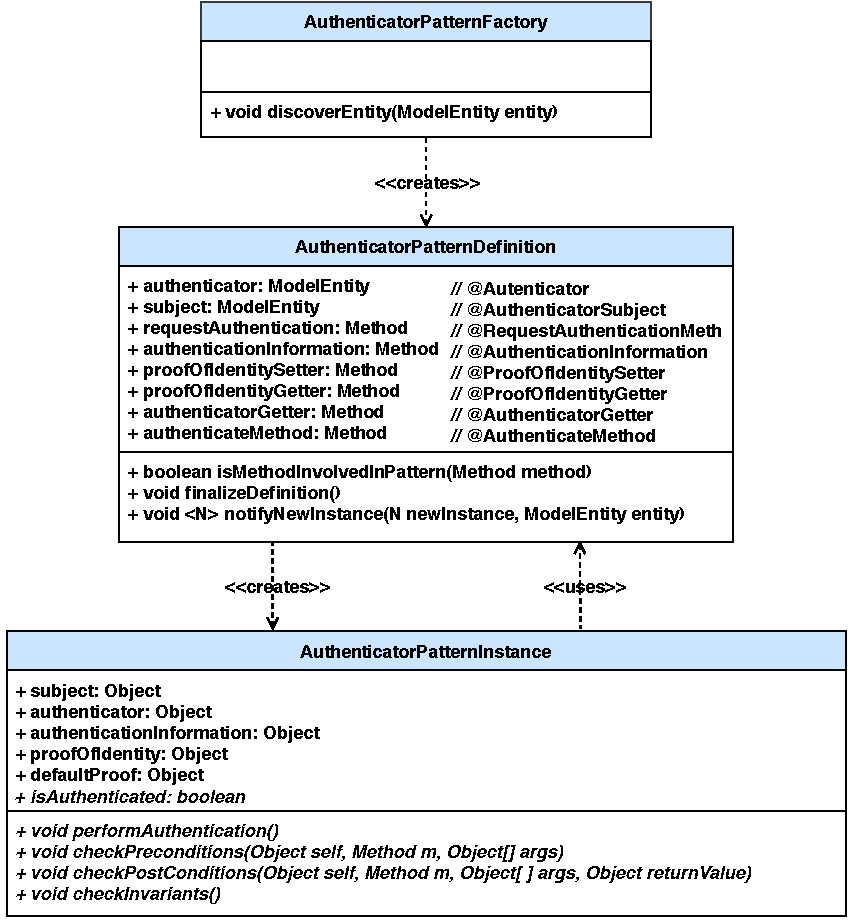
\includegraphics[width=0.8 \columnwidth]{utils/PAMELAAuthenticator_CD.pdf}
    \caption{PAMELA Authenticator pattern class diagram. Emphasized attributes and methods are the one referenced in Figure \ref{fig:AuthenticatorControlFlow}.}
    \label{fig:PAMELAAuthenticator_CD}
\end{figure}

To validate the implementation of our approach in PAMELA we propose an implementation of the \emph{Authenticator pattern} as a cyber-security contract. Figure \ref{fig:PAMELAAuthenticator_CD} presents the previous class structure in the case of the Authenticator pattern. Note that each attribute of the \mytexttt{AuthenticatorPatternDefinition} class has a corresponding annotation (displayed as a comment).

\begin{figure}
    \centering
    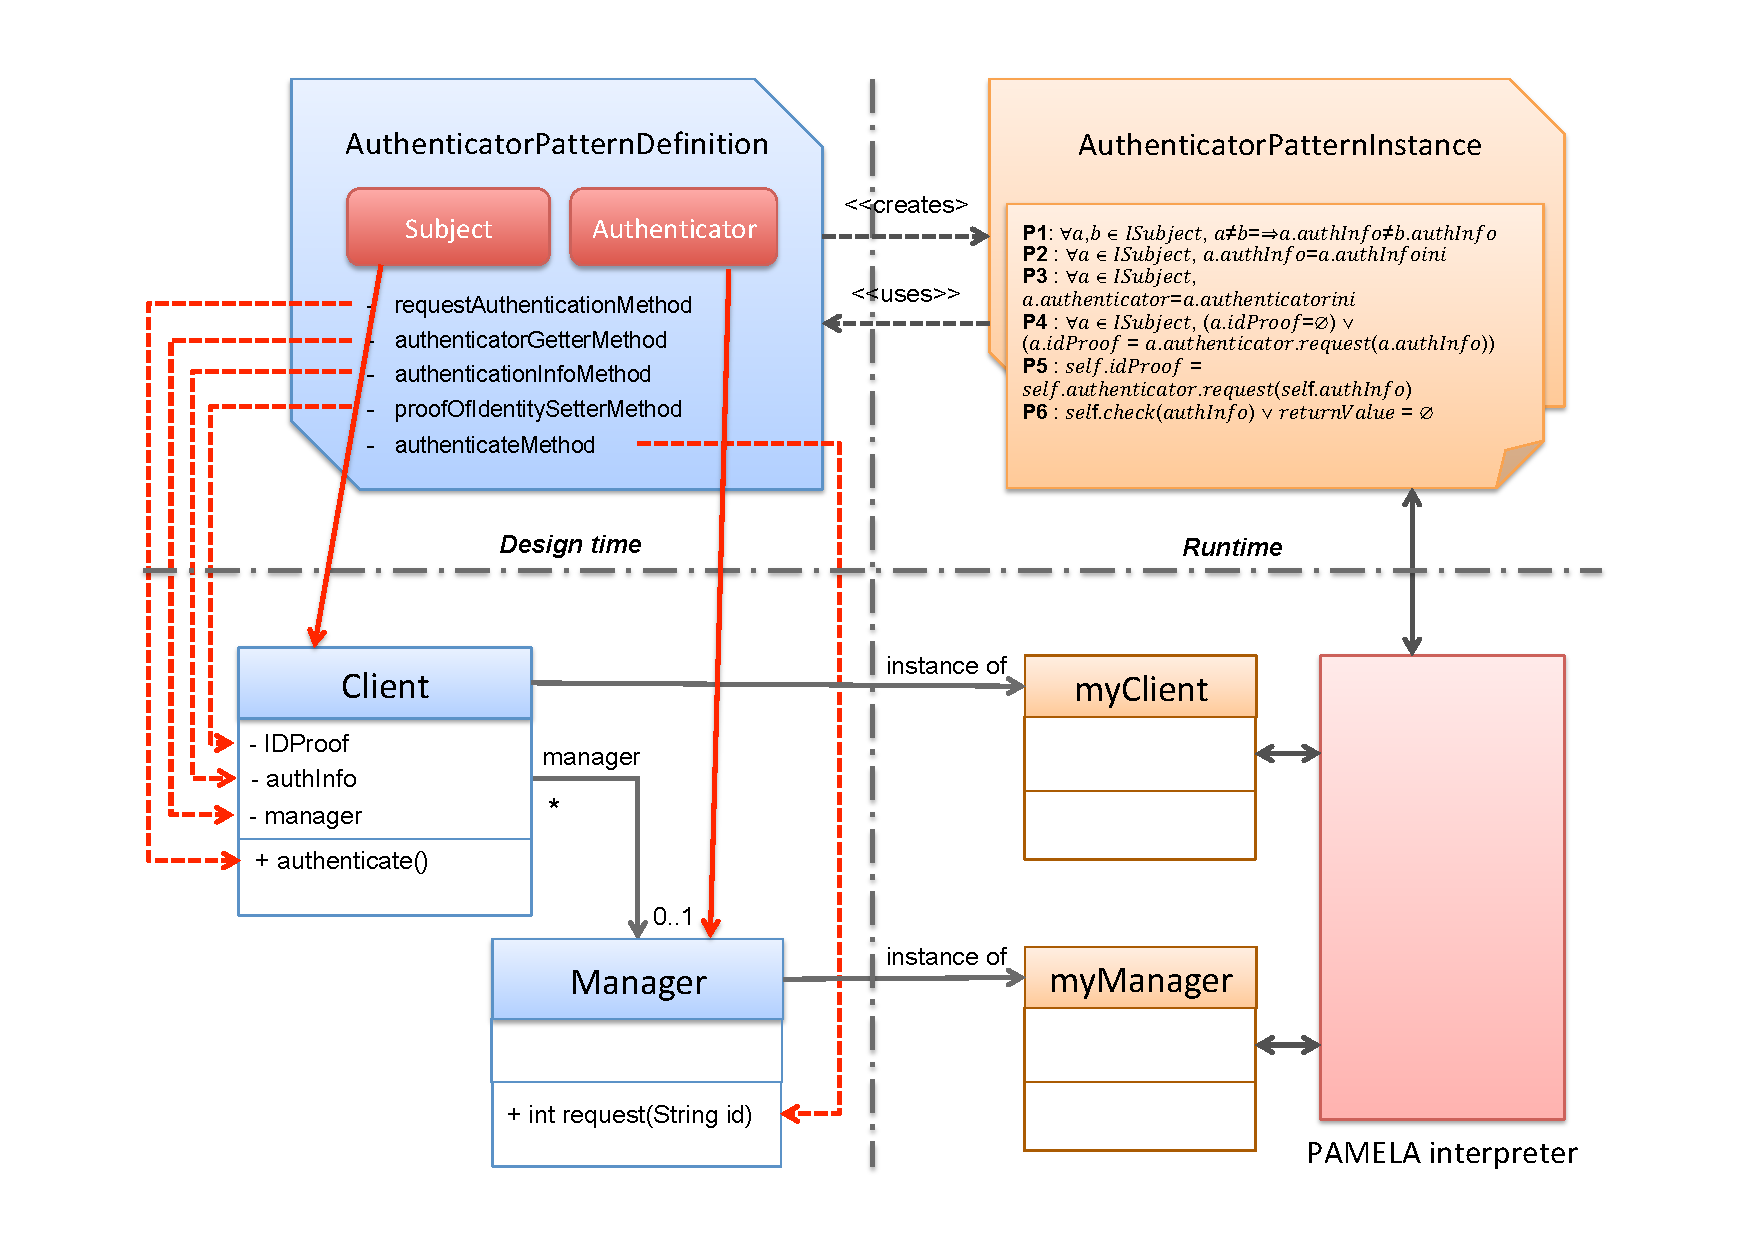
\includegraphics[width=1.0 \columnwidth]{AuthenticatorPattern4.pdf}
    \caption{PAMELA vision of the authenticator pattern}
    \label{fig:AuthenticatorPattern}
\end{figure}

Figure \ref{fig:AuthenticatorPattern} presents the composition of the \emph{Authenticator} pattern with an existing base of code. The  \emph{Authenticator pattern} requires the definition of two \emph{stakeholders} (\emph{Authenticator} role and \emph{Subject} role) which have to be played by instances of provided Java classes. A set of annotations coming with the \emph{security pattern} definition is used to explicit that roles (respectively \texttt{@Authenticator} and \texttt{@AuthenticatorSubject} annotations). The definition of the pattern also requires the distribution of responsibilities and relationships according to the underlying semantics of the pattern (here, the authentication concerns). The request authentication method is identified using the \texttt{@RequestAuthentication} annotation. In the same way, we must identify some responsibilities in the \texttt{Client} class: the method providing the  \emph{Authenticator} access, the method providing the authentication information, the method setting the proof of identity and the \mytexttt{authenticate()} method itself.

%With that implementation, contract assertions do not require to be explicitly defined by the programmer, but are inherent to the security pattern, and are encoded in plain Java code. From an operational point of view, the security pattern is reified as a Java instance, and maintains a statefull environment on which contract assertions may be defined.


The excerpt of code presented Figure \ref{fig:ExampleOfAuthenticatorPattern} shows how the Authenticator pattern is used by means of annotations to an existing base of code. An instance of the \texttt{Manager} class plays the \emph{Authenticator} role, while an instance of the \texttt{Client} class plays the \emph{Subject} role.

\begin{figure}
    \centering
\begin{lstlisting}[language=Java,basicstyle=\ttfamily\footnotesize]
@ModelEntity
@Authenticator(patternID = "MyPatternId")
public class Manager {

	@RequestAuthentication(patternID = "MyPatternId")
	public int request(@AuthenticationInformation(patternID = "MyPatternId", paramID = "id") String id) {
		return ...;
	}
}

@ModelEntity
@AuthenticatorSubject(patternID = "MyPatternId")
public class Client {

	public Client(Manager authenticator, String id) {
		...
	}

	@AuthenticationInformation(patternID = "MyPatternId", paramID = "id")
	public String getAuthInfo() {
		return ...;
	}

	@ProofOfIdentityGetter(patternID = "MyPatternId")
	public int getIDProof() {
		return ...;
	}

	@AuthenticatorGetter(patternID = "MyPatternId")
	public Manager getManager() {
		return ...;
	}

	@AuthenticateMethod(patternID = "MyPatternId")
	public void authenticate() {
		setIDProof(getManager().request(getAuthInfo()));
	}

	@RequiresAuthentication
	public void securedMethod() {
		...
	}
}
\end{lstlisting}
    \caption{Example showing how to use the Authenticator pattern defined as a PAMELA cyber-contract}
    \label{fig:ExampleOfAuthenticatorPattern}
\end{figure}

%\emph{Authenticator} pattern implementation is provided by a Java implementation gathering three classes representing a different conceptual level as defined in the Meta-Object Facility (MOF):
%\begin{itemize}
%    \item \texttt{AuthenticatorPatternFactory.java} (layer M2) : provides features to identify in byte-code at run-time the implementation of an \emph{Authenticator} pattern, on the basis of \texttt{patternId} identifier.
%    \item \texttt{AuthenticatorPatternDefinition.java} (layer M1) : represents an occurrence of \emph{Authenticator} pattern in supplied byte-code. This class has the responsability of maintaining links with classes and methods involved in pattern, as well as managing life-cycle of that pattern instances. 
%   \item \texttt{AuthenticatorPatternInstance.java} (layer M0) : represents an instance of \emph{AuthenticatorPatternDefinition} pattern. This class has the responsability of maintaining state of pattern instance, and managing  business logic as offered by the pattern.
%\end{itemize}

%In the context of \emph{Contract Programming}, this is the AuthenticatorPatternInstance class which has the responsability of defining and checking at run-time the different contract clauses (invariants, preconditions and postconditions). Note that contrary to the JML implementation of our approach, the programmer does not have to define the contract clauses, which are hard-coded in pattern implementation.

%\subsubsection{PAMELA \emph{Patterns} Caine}

%We chose to extend the PAMELA framework to include our notion of \emph{Pattern}, i.e. a composition of multiple classes, knwon as \emph{Stakeholders}, whose expected behavior is defined in a pattern contract, along with formal properties which must be ensured at run-time. More specifically, the implemented PAMELA \emph{Pattern} feature provides:
%\begin{itemize}
%    \item the ability to use existing plain Java code, without any restriction;  \emph{Pattern}
%    \item the ability to monitor the execution of the code;
%    \item the ability to offer extra structural and behavioral features, executed by the PAMELA interpreter, 
%    \item a representation of \emph{Patterns} as stateful objects. Such objects can then evolve throughout run-time and allow the computation of assertions using many paradigms (e.g., Linear Temporal Logic);
%    \item multiple extension points: ability to redefine or specialize an existing pattern, and ability to provide a new pattern definition.
%\end{itemize}

%\emph{Patterns} are defined in PAMELA using three classes, each representing a different conceptual level:
%\begin{itemize}
%    \item a \mytexttt{PatternFactory}. This class provides features to identify in the java byte-code, at run-time, the declared patterns.
%    \item a \mytexttt{PatternDefinition}. This class represents an occurrence of the pattern in the supplied byte-code. It has the responsibility of maintaining links with all classes and methods involved in the pattern, as well as managing the life-cycle of its \mytexttt{PatternInstances}.
%    \item a \mytexttt{PatternInstance}. This class represents the instance of a pattern at run-time. It is responsible for maintaining the pattern state and providing pattern behavior and contract enforcement.
%\end{itemize}

%To declare a \emph{Pattern} on an existing code, pattern elements, i.e. \emph{Pattern Stakeholders} and methods, need to be annotated with provided pattern-specific Java annotations. These annotations will then be discovered at run-time by the \mytexttt{PatternFactory} and stored in \mytexttt{PatternDefinition} attributes. 

%The figure \ref{fig:PAMELAAuthenticator_CD} presents the previous structure in the case of the Authenticator pattern. Note that all attributes of the \mytexttt{AuthenticatorPatternDefinition} class are associated with an annotation (displayed as commentaries).
%\begin{figure}
%    \centering
%    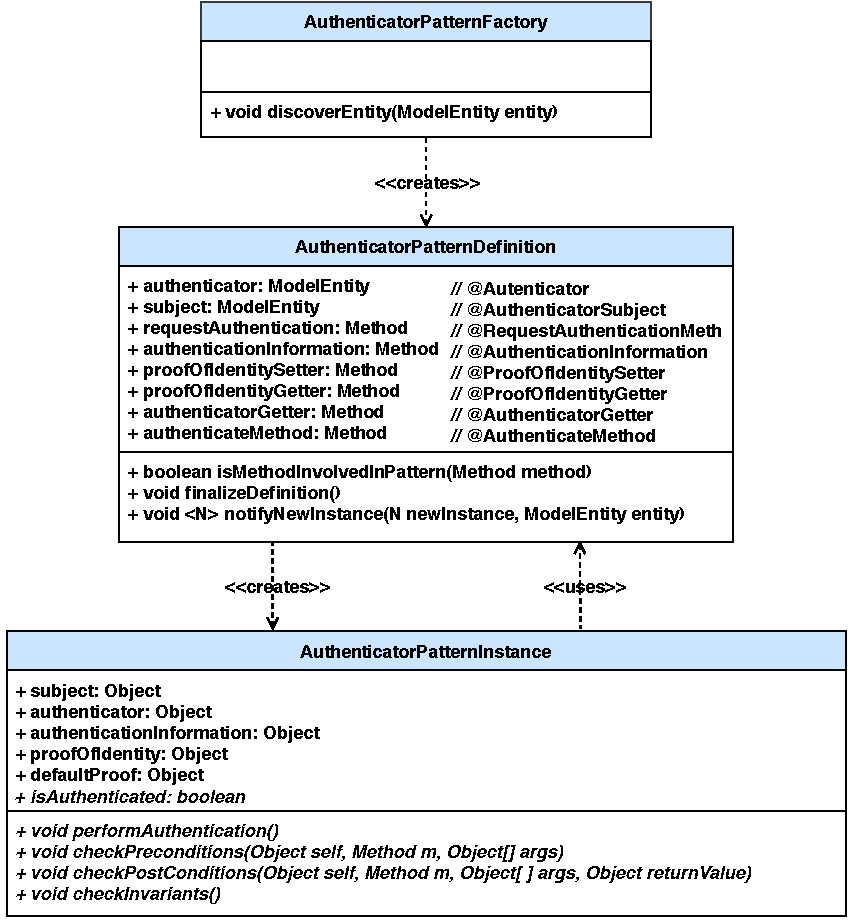
\includegraphics[width=1.0 \columnwidth]{utils/PAMELAAuthenticator_CD.pdf}
%    \caption{PAMELA Authenticator pattern class diagram}
%    \label{fig:PAMELAAuthenticator_CD}
%\end{figure}

At run-time, both functional code and security pattern logic, i.e pattern behavior and contract enforcement, are weaved by the PAMELA framework. 

%More specifically, \mytexttt{PatternDefinition} classes implement the \mytexttt{isMethodInvolvedInPattern} which returns \mytexttt{true} for all methods which need to be handled by the associated \mytexttt{PatternInstances}. This allows, for instance, for the pattern contract properties to be checked at run-time before and/or after any method of interest. In the case of the Authenticator pattern, the \texttt{AuthenticatorPatternInstance} objects will check the invariants of the pattern contract before and after every call to \emph{Subject} and \emph{Authenticator} classes. These checks are performed by the \texttt{checkInvariant} method. 

This implementation, unlike JML, provides a contract enforcement mechanism which is hard-coded within PAMELA \emph{Pattern} classes. This abstraction is closer to the requirements of the end-user, who may want to add an authentication mechanism to an existing code. The user only need to annotate his code and PAMELA will automatically handle the pattern business logic (both, pattern behavior and assertion checking).

\begin{figure}
    \centering
    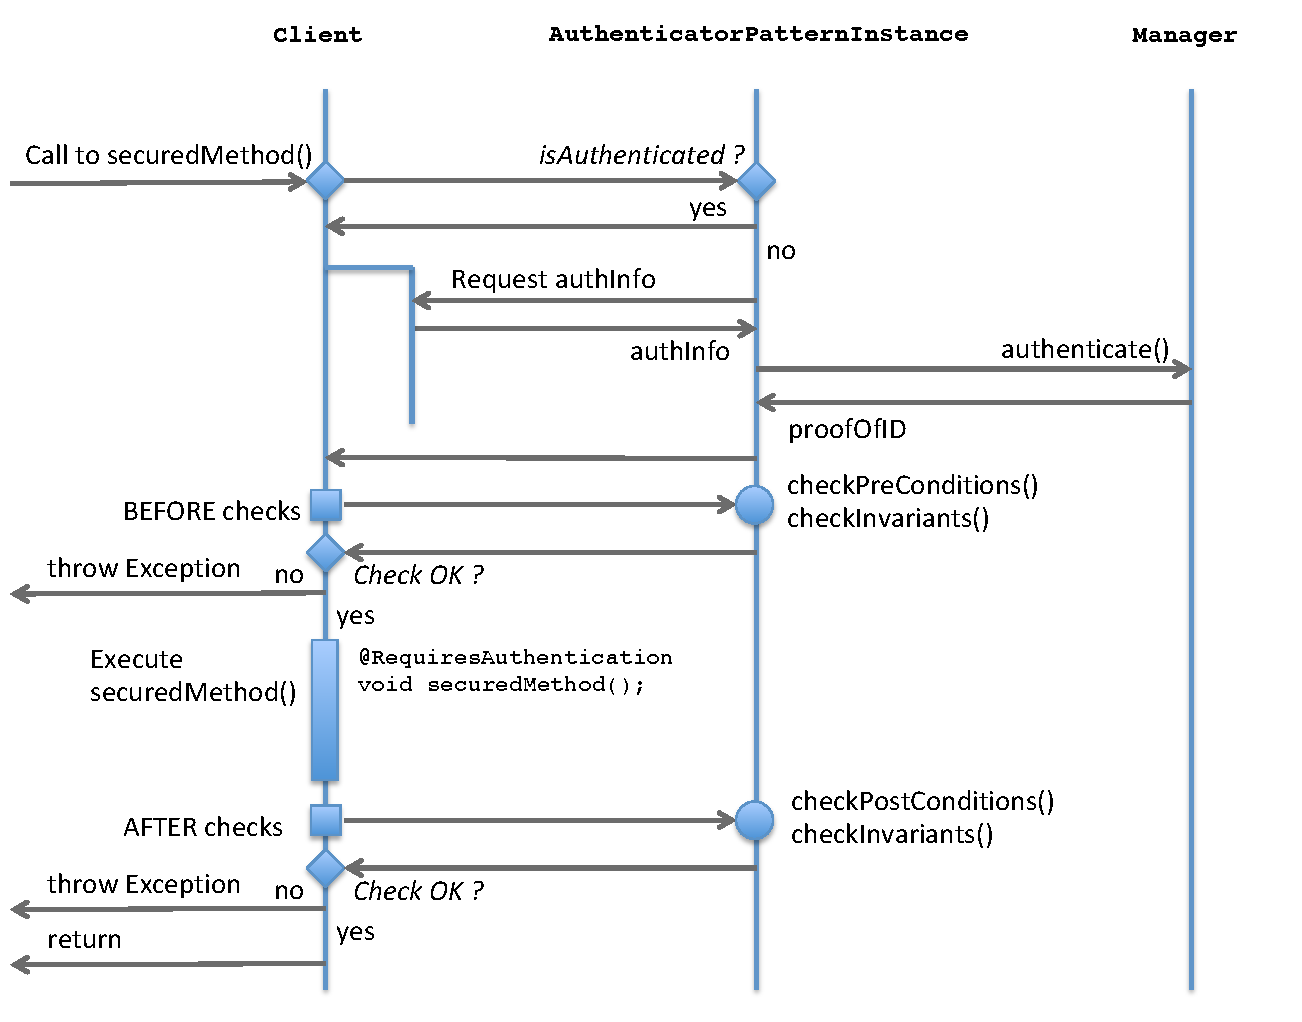
\includegraphics[width=1.0 \columnwidth]{AuthenticatorControlFlow.pdf}
    \caption{Authenticator control flow}
    \label{fig:AuthenticatorControlFlow}
\end{figure}

Figure \ref{fig:AuthenticatorControlFlow} depicts  the control flow of the execution of a method annotated with \mytexttt{@RequiresAuthentication}. 
This annotation is used to identify methods which must trigger the authentication process before being executed. The call will thus be handled as follows:
\begin{itemize}
	\item The method is identified as a method of interest because this method requires authentication.
	\item The method is passed to the relevant \mytexttt{AuthenticatorPatternInstance} (second object on the Figure) before the method execution.
	\item The authentication process is to be executed, because subject is not authenticated yet (\mytexttt{isAuthenticated} is \mytexttt{false}).
	\item Before executing the called method, contract invariants are checked (properties P1 to P4) via the \mytexttt{checkInvariants()} call. If a clause breach is detected, an exception is thrown and the method is not executed. This is also at this time that preconditions are checked (method \mytexttt{checkPreConditions}).
	\item The method is invoked.
	\item The method is once again passed to the \mytexttt{AuthenticatorPatternInstance} after the method execution. Contract invariants are checked. If a clause breach is detected, an exception is thrown. Similarly,  post-conditions are checked (method \mytexttt{checkPostConditions}).
	\item Finally, the result of the method is returned to the caller.
\end{itemize}

%PAMELA implementation results and lessons learned
\subsection{Lessons learned from experiments}

% lessons learned regarding the challenges of the introduction
The two experiments emphasize that the formal behavioral definition of security contracts is an efficient approach to provide several implementations based on our design by contract definition.

The JML experiment highlights the limitations of this DbC implementation for security pattern contract definition. DbC implementations are too limited and fail to express properties requiring multiple class instances or an evolving pattern state. This justifies  the necessity to extend the scope of contract definitions to more complex contracting parties, such as sets of classes. 

These limitations are overcome with the PAMELA approach which provides the ability to freely build models based on multiple  classes with their own semantics and behavioral code.
In this case, our security cyber-contracts are applied at the top of the set of classes used in the security pattern.  
%The PAMELA experiment points out the capacity to allow (i) the verification, at run-time, of clauses involving universal and existential quantifiers on a set of instances and (ii) the support of temporal clauses on stateful instances. 

Regarding the challenges we wanted to target, PAMELA provides an efficient and easy framework to apply security patterns using Java annotations . This can be done at a very early stage of design process of a software component, but this framework can also be applied on legacy source code beeing annotated.

Securing existing code remains a difficult task but our proposal, based on both formal behavioral contract and run-time property enforcement, enforces the security of software components.

%\begin{itemize}
%    \item Structural boundary limitations observed with JML do not apply here, because a pattern may involve an arbitrary instances of different classes playing a role.
%    \item PAMELA offers a run-time access to all instances of patterns and their definitions, allowing verification of clauses involving universal and existential quantifiers. 
%    \item Because pattern instances are statefull, we may consider temporal assertions (such as Linear Temporal Logic formalism).
%\end{itemize}

%Application to \emph{SecurityPatterns} offers the way to provide a secured run-time environment where calls to functional code are dynamically weaved with security pattern internal policy, and are guarded with run-time verification of some security assertions.

%\subsection{Evaluation}

%\subsubsection{Cases}

%To evaluate our approach, we conducted a set
%of experiments on two cases: ...

%\subsubsection{Effectiveness}

%To determine the effectiveness of the approach, we measure the ... of each case. In Figure X and Figure Y, we present the results of ... The figures show the measurements of the security metrics after/corresponding to ...

%As a threat to validity, we acknowledge that we only performed a relative small number of experiments and further study with more complex systems is required to derive stronger conclusions. Nevertheless, from the results of our experiments we can observe that ... increases/decreases the security level of the system as demonstrated in Figure X and Figure Y. In addition, we observe that ...

%*
%\subsubsection{JML experiment}

%A first experimentation has been made with the support for JML annotations in OpenJML framework, in a context of \emph{Design by Contract} programming. We started from an existing base of functional code, implementing the concepts of \emph{Manager} and \emph{Client}, and assuming the choice of \emph{Authenticator} security pattern, we've added JML clauses (invariants, pre and post conditions) as java annotations in related classes and methods.

%The application has two classes: A \emph{Client} class and a \emph{Manager} class. Clients are identified by a unique integer that allows them to obtain a security token from the Manager. The Manager assigns the -1 token to non-privileged clients and a specific value, which changes with each execution of the application, to privileged clients. This corresponds to the \emph{Authenticator} pattern. The \emph{Manager} also has a secure resource (a string here). To secure it, the Authorization pattern is implemented. To be able to modify it, clients must make a request to the manager which checks the client’s security token. If this one is correct, the request is processed (read or write the string), otherwise, it is ignored. The class diagram is given in the figure \ref{fig:manager_client}. The code also contains the JML annotations that correspond to the contract clauses of the two patterns.

%\begin{figure}
%    \centering
%    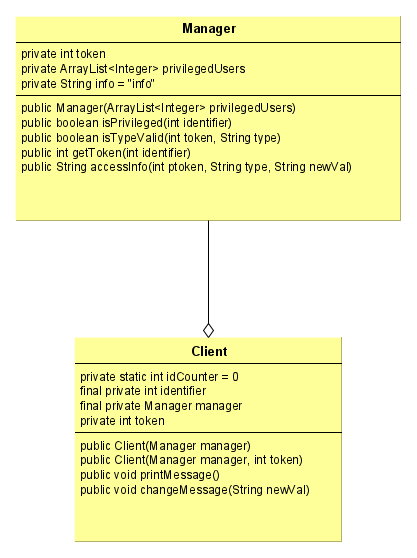
\includegraphics[width=.7 \columnwidth]{utils/Prototype.png}
%    \caption{Functional code for Authenticator pattern}
%    \label{fig:manager_client}
%\end{figure}

%For execution, three clients and a manager are created. The first one is known to the manager as privileged. The second is not privileged. The third one does not authenticate but has the security token (it is for example the case of an attacker who would have succeeded in stealing the security token). Each of these clients then tries to change the value of the resource.

%When the code is executed without JML assertions, the results are final. The third user manages to change the value of the resource. This behavior is perfectly normal since he has the right security token. Indeed, the simple implementation of patterns as described in the UML class diagrams in section 1.3 does not secure the application. In particular, it does not protect the system against identity theft. However, when JML assertions are enabled, the problem is detected as an invariant breach and the program stops.

%Thus, we can see that even in a really simple case, the simple implementation of security patterns is not enough to guarantee the security of the application. However, the verification of the formal contracts defined previously allows to protect against more attacks.

%However, the OpenJML option is not perfect. Indeed, since JML is defined for specification purposes and according to the DbC approach, it is not designed for security. Following limitations are observed:
%\begin{itemize}
 %   \item Some clauses does refer to an assembly of classes, and not a unique class, making impossible to be expressed using JML. A possible workaround is to refactor initial code, but it contradicts our initial requirement to secure existing functional code without being intrusive.
 %   \item For the same reasons, it is really difficult to handle delegation contracts.
 %   \item For some clauses, we need to reference all the instances of a particular concept, and not only the current one (eg P1: uniqueness of Authentication information/Subject pairs).
%    \item Some clauses require a temporal window to be expressed, which is not possible yet.
%\end{itemize}

%For those reasons, we have decided to experiment another approach related to Java annotations, the PAMELA framework \cite{}.

% Sylvain
% Ce serait bien de voir des annotations JML (sur la base d'un code déjà existant)
% Ce serait bien de faire le lien entre ces annotations et les clauses de contrat qu'on a mises en évidence avant, afin de voir ce qu'on peut exprimer, et ce qu'on ne peut pas
% Expliciter ensuite toutes les limitations, et pourquoi on ne peut pas le faire avec JML


% References sur PAMELA

% TODO: est ce qu'on présente PAMELA comme une implem' du MOP (Meta Object Protocol) ?

%PAMELA offers several features, such as:
%\begin{itemize}
%    \item Full life-cycle management of model objects (construction, destruction)
 %   \item Multiple inheritance and traits programming
  %  \item Embedding management and cloning support
   % \item Integrated fine notification support
    %\item Persistence support
    %\item Object graph closure computation, comparison and diff-merge support
    %\item Meta-programming support
    %\item Multi-level UNDO/REDO stack
%\end{itemize}

